\documentclass[12pt]{article}

\usepackage[english]{babel}
\usepackage[utf8]{inputenc}
\usepackage{fancyhdr}

\usepackage[margin=1in]{geometry}
\usepackage{pgf}
\usepackage{pgfplots}
\usepackage{siunitx}
\usepackage{tikz}
\usepackage{float}
\usepackage{amsmath}
\usepackage{enumitem}

\usepackage[font=small,labelfont=bf]{caption}
\usepackage{pstricks-add}
\usepackage{pgfplotstable}
\usepackage[nodisplayskipstretch]{setspace}

\usetikzlibrary{scopes}
\usetikzlibrary{angles,quotes}
\usetikzlibrary{calc}
\pgfplotsset{compat=1.5}
\graphicspath{ {/} }

\newcommand*{\I}{\imath}
\newcommand*{\J}{\jmath}
\newcommand{\norm}[1]{\lvert #1 \rvert}

\setlist[enumerate, 1]{label=\alph*.}


\begin{document}
\sisetup{per-mode=symbol}

\begin{titlepage}
    \begin{center}
        \vspace*{1cm}
        \textbf{The Oscilloscope}

        \vspace{0.5cm}
        Lab: 04

        \vspace{1cm}

        \textbf{Jaden Moore}

        \vfill

        Orange Coast College\\
        Physics A280L\\
        March 22nd, 2021

    \end{center}
\end{titlepage}

\pagestyle{fancy}
\fancyhf{}
\setlength{\headheight}{15pt}
\lhead{The Oscilloscope}
\rhead{Lab: 04}
\cfoot{\thepage}

\section{Introduction}
In this lab, we use an oscilloscope to analyze the motion and frequency of multiple voltage signals over time. Through the graph obtained from an oscilloscope, we will be able to identify the period, frequency, peak-to-peak voltage, and amplitude of the voltage signal. We then compare the measured frequency with the theoretical frequency of the signal to obtain a percent error in our experimental values.

\section{The Oscilloscope}
Consider the graphs of voltage signals below. From analyzing the graphs, we obtain the period, frequency, peak-to-peak voltage, and the amplitude of the original voltage signal read by the oscilloscope. We then compare the theoretical frequency with the experimental frequency gathered from the graph and then compute the percent error. The data in this lab is from the Academo: Virtual Oscilloscope simulation.

\subsection{Voltage Signal 1}
\begin{figure}[H]
    \begin{center}
        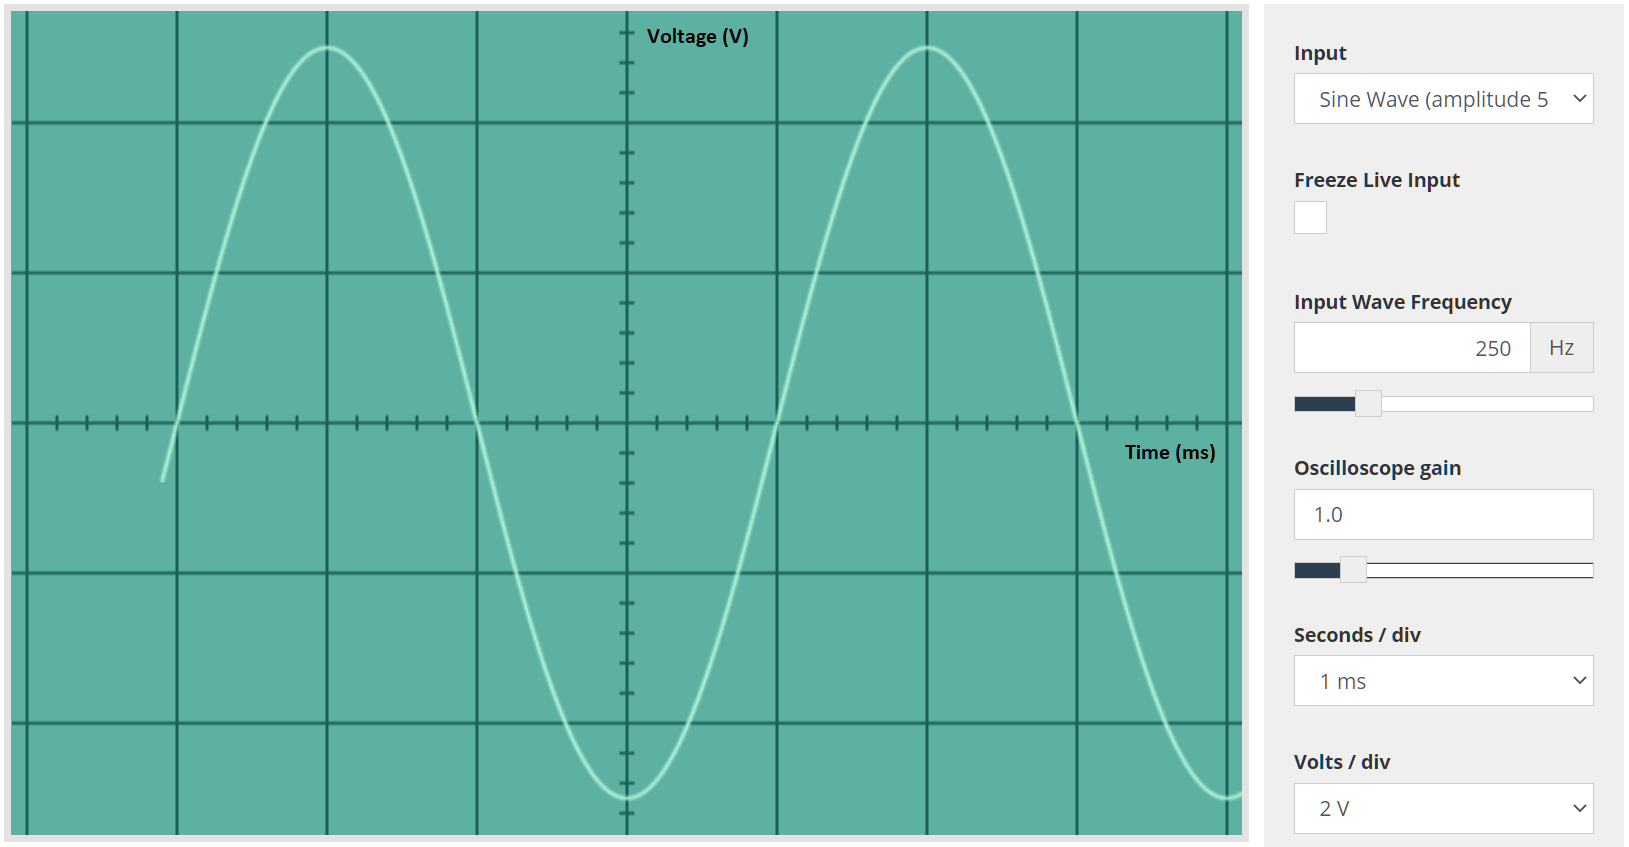
\includegraphics[scale=0.6]{Figure-1.png}
        \caption { Voltage Signal 1: Sine Wave}
    \end{center}
\end{figure}

\newpage

Below is the properties of Figure 1:

\begin{equation*}
    \begin{split}
        \text{Period} & = \SI{4}{div}\left(\frac{\SI{1}{ms}}{\SI{1}{div}}\right) = \SI{4}{ms} \\
    \text{Frequency} & = \frac{1}{period} =\frac{1}{\SI{4}{x10^{-3} s}} = \SI{250}{Hz} \\
        \text{Peak-to-Peak Voltage} & = \left(\frac{\SI{5}{div}}{\SI{1}{}}\right)\left(\frac{\SI{2}{volts}}{\SI{1}{div}}\right) = \SI{10}{volts} \\
        \text{Amplitude} & = \left(\frac{\SI{2.5}{div}}{\SI{1}{}}\right)\left(\frac{\SI{2}{volts}}{\SI{1}{div}}\right) = \SI{5}{volts} \\
        \text{\% Error of Frequency} & = \left(\frac{\SI{250}{Hz} - \SI{250}{Hz}}{\SI{250}{Hz}}\right)100 = 0 \text{\% Error}
    \end{split}
\end{equation*}

\subsection{Voltage Signal 2}
\begin{figure}[H]
    \begin{center}
        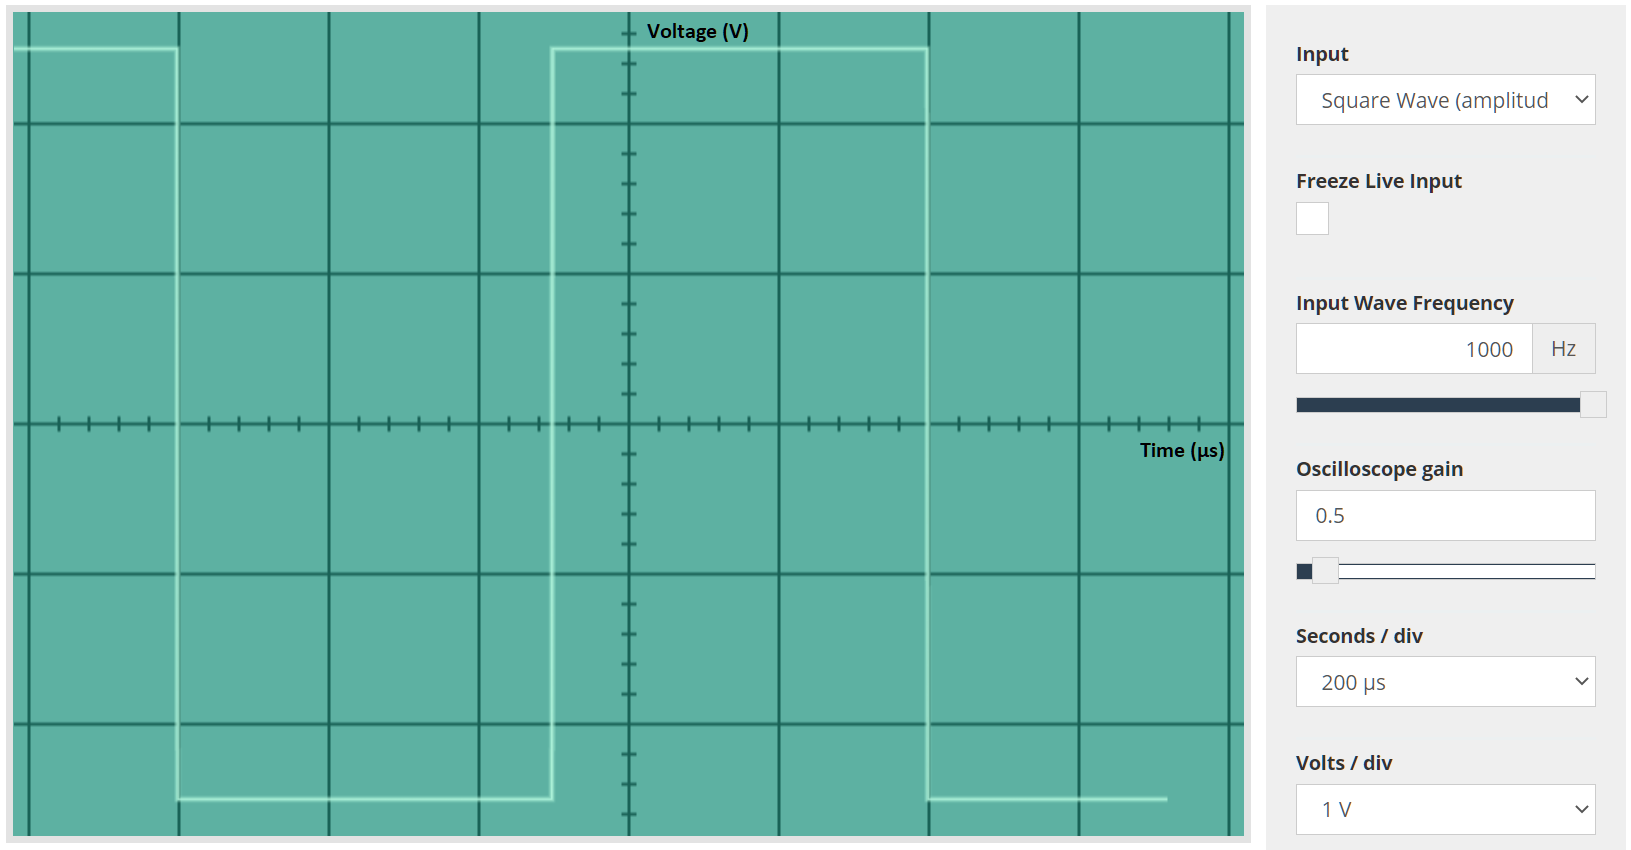
\includegraphics[scale=0.6]{Figure-2.png}
        \caption { Voltage Signal 2: Square Wave 1}
    \end{center}
\end{figure}

\newpage

Below is the properties of Figure 2:

\begin{equation*}
    \begin{split}
        \text{Period} & = \SI{5}{div}\left(\frac{\SI{200}{\us}}{\SI{1}{div}}\right) = \SI{1000}{\us} \\
    \text{Frequency} & = \frac{1}{period} =\frac{1}{\SI{1000}{x10^{-6} s}} = \SI{1000}{Hz} \\
        \text{Peak-to-Peak Voltage} & = \left(\frac{\SI{5}{div}}{\SI{0.5}{}}\right)\left(\frac{\SI{1}{volts}}{\SI{1}{div}}\right) = \SI{10}{volts} \\
        \text{Amplitude} & = \left(\frac{\SI{2.5}{div}}{\SI{0.5}{}}\right)\left(\frac{\SI{1}{volts}}{\SI{1}{div}}\right) = \SI{5}{volts} \\
        \text{\% Error of Frequency} & = \left(\frac{\SI{1000}{Hz} - \SI{1000}{Hz}}{\SI{1000}{Hz}}\right)100 = 0 \text{\% Error}
    \end{split}
\end{equation*}

\subsection{Voltage Signal 3}
\begin{figure}[H]
    \begin{center}
        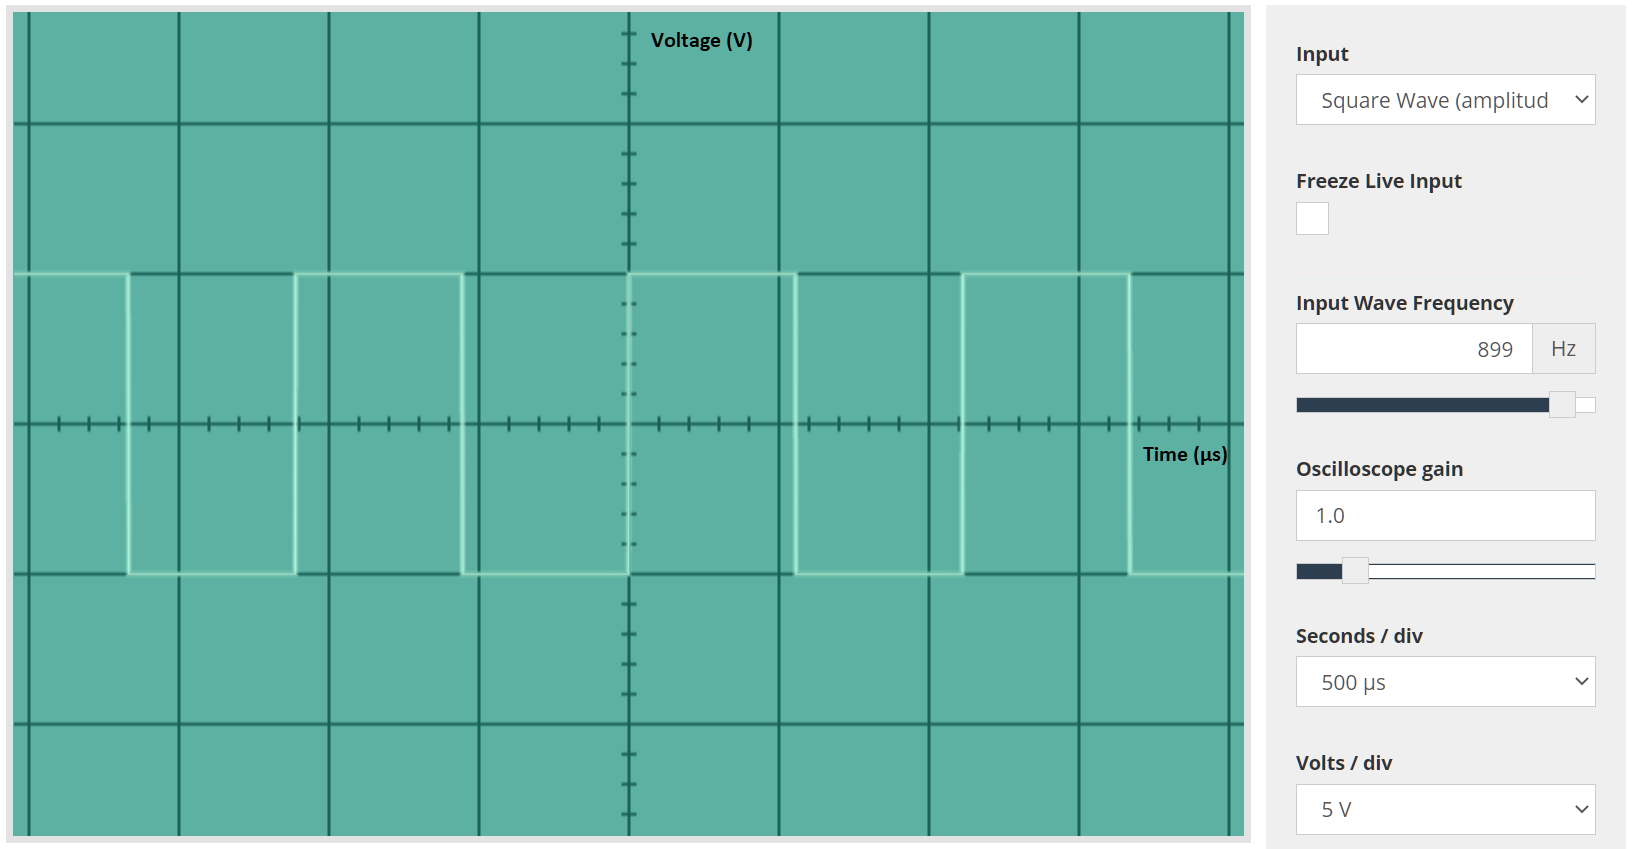
\includegraphics[scale=0.6]{Figure-3.png}
        \caption { Voltage Signal 3: Square Wave 2}
    \end{center}
\end{figure}

\newpage

Below is the properties of Figure 3:

\begin{equation*}
    \begin{split}
        \text{Period} & = (\SI{2.2}{div})\left(\frac{\SI{500}{\us}}{\SI{1}{div}}\right) = \SI{1100}{\us} \\
    \text{Frequency} & = \frac{1}{period} =\frac{1}{\SI{1100}{x10^{-6} s}} = \SI{909.1}{Hz} \\
        \text{Peak-to-Peak Voltage} & = \left(\frac{\SI{2}{div}}{\SI{1}{}}\right)\left(\frac{\SI{5}{volts}}{\SI{1}{div}}\right) = \SI{10}{volts} \\
        \text{Amplitude} & = \left(\frac{\SI{1}{div}}{\SI{1}{}}\right)\left(\frac{\SI{5}{volts}}{\SI{1}{div}}\right) = \SI{5}{volts} \\
        \text{\% Error of Frequency} & = \left(\frac{\SI{909.1}{Hz} - \SI{899}{Hz}}{\SI{899}{Hz}}\right)100 = 1.12 \text{\% Error}
    \end{split}
\end{equation*}

\subsection{Voltage Signal 4}
\begin{figure}[H]
    \begin{center}
        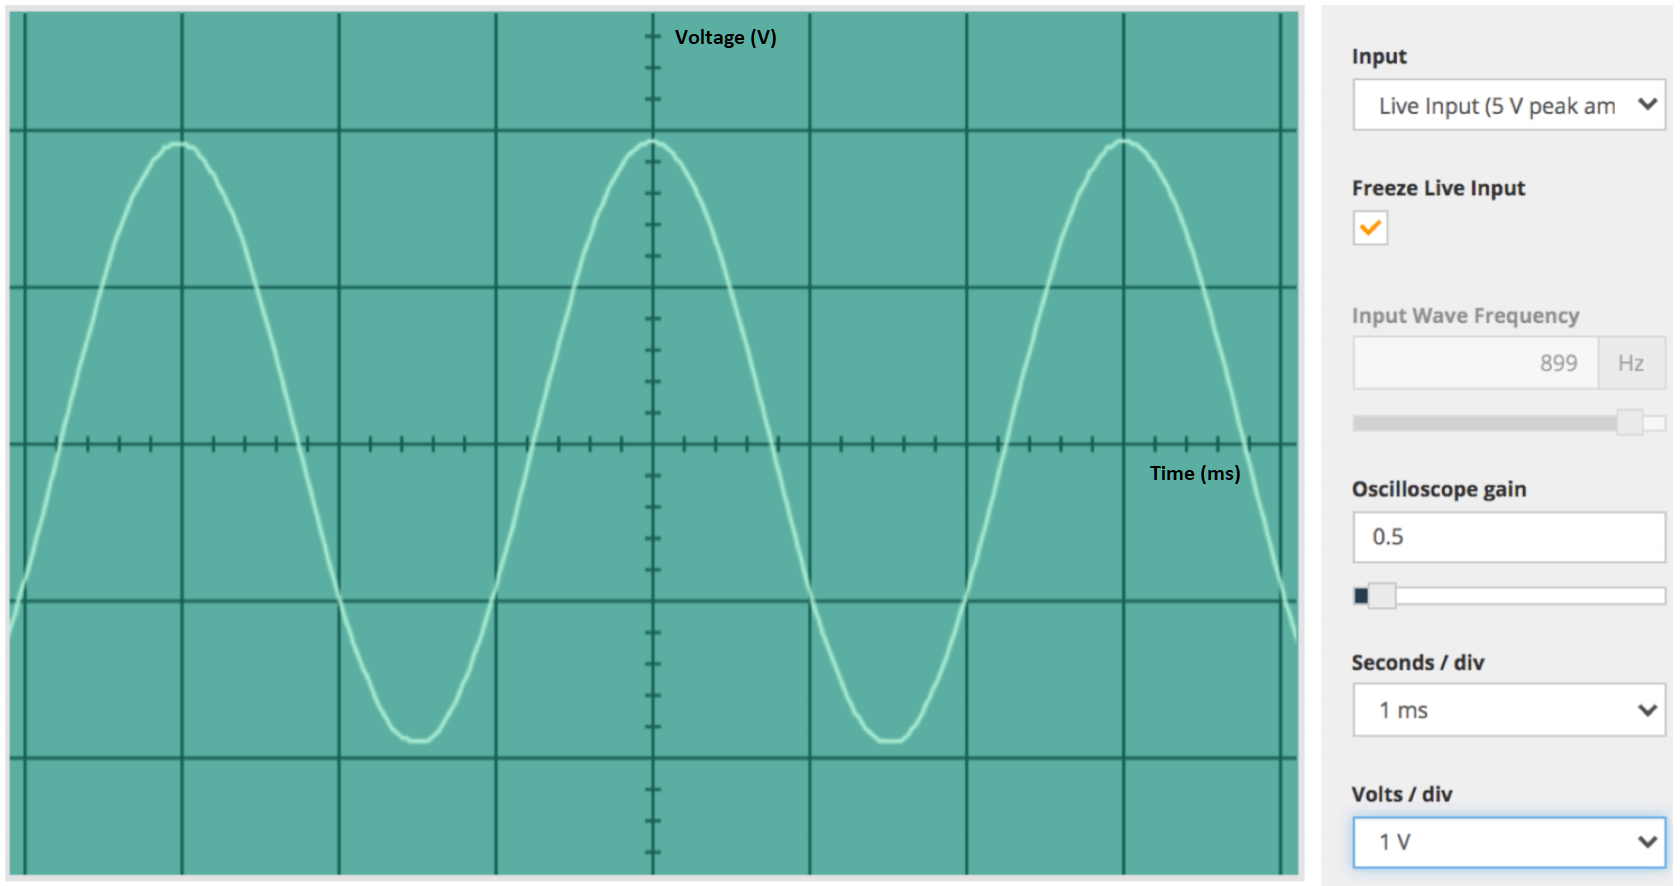
\includegraphics[scale=0.6]{Figure-4.png}
        \caption { Voltage Signal 4: Voice Wave}
    \end{center}
\end{figure}

\newpage

Below is the properties of Figure 4:

\begin{equation*}
    \begin{split}
        \text{Period} & = (\SI{3}{div})\left(\frac{\SI{1}{\ms}}{\SI{1}{div}}\right) = \SI{3}{\ms} \\
    \text{Frequency} & = \frac{1}{period} =\frac{1}{\SI{3}{x10^{-3} s}} = \SI{333.3}{Hz} \\
        \text{Peak-to-Peak Voltage} & = \left(\frac{\SI{3.8}{div}}{\SI{0.5}{}}\right)\left(\frac{\SI{1}{volts}}{\SI{1}{div}}\right) = \SI{7.6}{volts} \\
        \text{Amplitude} & = \left(\frac{\SI{1.9}{div}}{\SI{0.5}{}}\right)\left(\frac{\SI{1}{volts}}{\SI{1}{div}}\right) = \SI{3.8}{volts} 
    \end{split}
\end{equation*}

\section{Conclusion}
It follows from the lab that a lot of important information about a voltage signal can be captured by an oscilloscope. In this lab, we obtained important data related to the voltage wave depicted by the graph such as the period, frequency, peak-to-peak voltage, and amplitude. These values allow us to get a better understanding of the voltage waves emitted by a circuit or sound for example. The greatest obstacle was calculating the divisions between the various maxima and minima of the wave to obtain accurate data about the wave. The biggest takeaway was gaining a better understanding of how scientist use tools like an oscilloscope to identify frequencies of voltage waves and their types by analyzing the graph of their waves.
\end{document}
